\section{Implementation} Second step of adopting the automation practices is setting up the processes using chosen tools. The implementation goal is to pro


\subsection{Containerization}  I have adopted the containerization using Docker for a use in CI/CD pipeline. The Dockerfile simply contains the instruction for building a Docker images. It composed of specific commands which tell how to build the image. A Docker image is a read-only file containing a set of instructions. When these instructions are executed, a Docker container is created. 
%https://www.simplilearn.com/tutorials/docker-tutorial/what-is-dockerfile


\begin{lstlisting}[language=Octave, caption=Dockerfile]
FROM node:latest as build
WORKDIR /app
COPY package*.json ./
RUN yarn
COPY ./ .
RUN yarn run build

FROM nginx
RUN mkdir /app
COPY --from=build /app/dist /app
COPY nginx.conf /etc/nginx/nginx.conf
\end{lstlisting}

\noindent Dockefile showed on listing 5.1 contains installing dependencies on the fifth row and application bundling on the six's row using Yarn and also adding Nginx configuration from the \texttt{nginx.conf} file on the last row, which defines parameters like hostname, listen port and others.



\subsection{CI/CD pipeline configuration} CI/CD pipeline is a set of steps that are executed when the pipeline was triggered.\\
Listing 5.2 shows all the stages of the CI/CD pipeline. First two stages where configured by Ing. Oldřich Malec with the first setup of the frontend projects. Download stage installs all the dependencies required for the application run. Codestyle stage provides linting of the source code. Other three stages I have implemented in this thesis.
\begin{lstlisting}[language=Octave, caption=Gitlab CI/CD stages]
stages:
  - download
  - codestyle
  - test
  - build
  - deploy
\end{lstlisting}

\noindent GitLab provides the visualization of the pipeline steps and allows to execute any steps manually as well as monitor the log of any job from the pipeline. Figure 5.1 shows how the passed pipeline looks in the BI-DBS portal frontend.

\begin{figure}[ht]
\centering
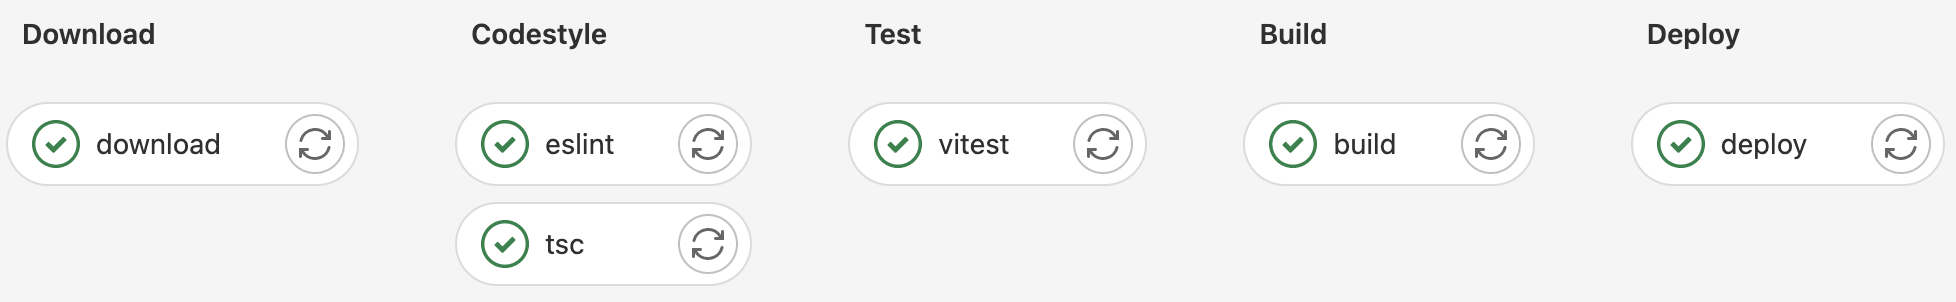
\includegraphics[scale=0.377]{../png/pipeline.png}
\caption{CI/CD pipeline in GitLab}
\end{figure}

\noindent The pipeline stages are executed from left to right and if any of the stages fails all the other ones will be skipped. It helps to avoid pointless running of jobs, because the stages are put in the way that they depend on the result of the previous ones. 




\subsubsection{Test} Test stages contains one job which I have named vitest, because it executes unit tests implemented using Vitest framework which will be introduced in the six's chapter. For running the tests I have used Yarn, which provides the tests execution by running just one command which is added to script section on the line fifteen of the listing 5.3. 
\begin{lstlisting}[language=Octave, caption=Test stage in the CI/CD pipeline]
.image_template: &image
  image: $CI_REGISTRY/ict/images/alpine/ci:3.16
  before_script:
    - apk add -U nodejs yarn

.cache_pull_template: &cache
  key: $CI_COMMIT_REF_SLUG
  paths:
    - node_modules/
    
vitest:
  <<: *image
  stage: test
  script:
    - yarn run test
  cache:
    <<: *cache

\end{lstlisting}

\noindent For the tests execution setup in the pipeline I have used image and cache pull templates, which were already prepared and used for the download and codestyle stages.




\subsubsection{Build} Build stage is focused on building an image and adding it to the GitLab container registry of the project. I have used the faculties image containing buildah and buildah itself for the script which is shown in listing 5.4. Command from the row number seven will create the image and the next command from the row number eight will upload it to GitLab registry.\\

\begin{lstlisting}[language=Octave, caption=Build stage in the CI/CD pipeline]
build:
  image: $CI_REGISTRY/ict/images/buildah:v1
  stage: build
  variables:
    IMAGE_TAG: $CI_REGISTRY_IMAGE:$CI_COMMIT_REF_NAME
  script:
    - buildah build --squash --tag $IMAGE_TAG -f Dockerfile
    - buildah push $IMAGE_TAG
  only:
    - master
\end{lstlisting}

\noindent The last two rows of the listing define the only branch for which this job will be executed. The BI-DBS frontend does not have a production version yet. Therefore I have decided to create the environment for deploying the application for testing during the development process. The changes are configured to be built and deployed only from a master branch.

\paragraph*{Change in the deployment flow.} In the current application the master branch is configured to be a production state branch, while the branch named devtest is used for deployment to the test environment. From my implementation there is a change that is going to be established to the new project, when a master will be to representing a state of a test environment and the deployment to the deployment to the production environment will be implemented by using tags for the master branch with the application version. This approach has several advantages for the BI-DBS frontend project.

\begin{itemize}
\item \emph{Easier maintenance and  flexibility.} Using just one branch reduces complexity of merging branches and maintenance of multiple branches. 

\item \emph{Simulation of a production. } The master branch state always represents a state which is very similar to the production state. It means that developers can see how their changes would behave in the production. This implies a few next benefits.
\begin{itemize}
    \item It allows to thoroughly test the application before deploying to the\\ production.
    \item Provides a possibility to give faster and higher quality feedback on code and changes.
\end{itemize}
\end{itemize}

\subsubsection{Deploy} When it comes to deploy stage, it means that the application went though all the previous pipeline stages and is ready to be deployed. The deployment process of the CI/CD pipeline is composed of execution of the deployment script by the server. For the connection to the server GitLab uses CI/CD variables which allow securely storing sensitive data, which need to be used in the pipeline like for example deployment user showed on line number six of listing 5.5.


\begin{lstlisting}[language=Octave, caption=Deploy stage in the CI/CD pipeline]
deploy:
  stage: deploy
  dependencies:
    - build
  script:
    - ssh -A "${DEPLOYER_IP_ADDRESS}" -l ${DEPLOYER_USER} 'cd ~/dbs-frontend && git pull && cd ./.docker/server && bash deploy-dbs-frontend.sh'
  only:
    - master
\end{lstlisting}

\

\noindent \textbf{Deployment script.} In a difference with a current application the deployment script is now being versioned and stored in the git remote repository instead of a server only. Therefore, before the script execution the server pulls all the changes from the remote repository.\\ The deployment script, which is shown in listing 5.6 contains few steps such as pulling Docker image from the GitLab created in the build stage on the row number seven, then running a container defined and configured in the \texttt{docker-compose.yaml} file showed in listing 5.7. Then the script provides the "healthcheck" of the environment, which is a check for controlling the availability of the resource. And finally on the last two rows script starts showing the logging of the container and removes unused images from the local docker host for removing the disk space.

\begin{lstlisting}[language=Octave, caption=Deployment script]
#!/bin/bash

set -e

HEALTHCHECK_URL="https://dbs3.fit.cvut.cz"

docker compose pull
docker compose up -d

attempt_counter=0
max_attempts=30

until $(curl --output /dev/null --silent --head --fail "${HEALTHCHECK_URL}")
do
  if [ "${attempt_counter}" -eq "${max_attempts}" ]
  then
    echo "Max attempts reached"
    docker logs dbs-microservices-frontend
    exit 1
  fi

  attempt_counter=$(($attempt_counter+1))
  echo "Waiting for URL ${HEALTHCHECK_URL}... (${attempt_counter}/${max_attempts})"
  sleep 2
done

docker logs dbs-microservices-frontend
docker image prune --force
\end{lstlisting}

\

\noindent Listing 5.7 shows the file which is used for the configuration and run of container. Firstly, it defines the image which will be dowloaded from the GitLab. Secondly it defines a network, that allows the communication with the services from the same network. Thirdly it tells the service to restart automatically in it case it stops for any reason. Then it specifies the container ad host names as well as ports mapping. Finally it gives a label, which can be used for the service identification as a microservice of the application.

\begin{lstlisting}
version: '3.8'
services:
  dbs-frontend:
    image: 'gitlab.fit.cvut.cz:5000/dbs/dbs-frontend:master'
    networks:
      - internal
    restart: always
    container_name: 'dbs-microservices-frontend'
    hostname: 'dbs3.fit.cvut.cz.internal'
    ports:
      - '8080:80'
    labels:
      cz.cvut.fit.dbs.microservice: 'Frontend'
networks:
  internal:
    external: true
\end{lstlisting}